\documentclass{beamer}
\usefonttheme[onlymath]{serif}

\mode<presentation>
{
  \usetheme{Frankfurt}
  \usecolortheme{dove}  %% grey scale
  \useinnertheme{circles}
  % \setbeamercovered{transparent}
}

\hypersetup{
    colorlinks,
    citecolor=black,
    filecolor=black,
    linkcolor=black,
    urlcolor=blue
}
\usepackage{graphicx}
\usepackage{color}
\usepackage{changepage} % for adjustwidth
\usepackage{xcolor}
\usepackage[most]{tcolorbox}

\graphicspath{ {./imgs-lattices} }

\setbeamertemplate{itemize}{$\circ$}
\setbeamertemplate{itemize items}{$\circ$}

\beamertemplatenavigationsymbolsempty %% no navigation bar

\setbeamertemplate{footline}{\hspace*{.1cm}\scriptsize{
\hspace*{50pt} \hfill\insertframenumber/\inserttotalframenumber\hspace*{.1cm}\vspace*{.1cm}}}

% paint red background to slides that I may end up removing
\newenvironment{mayberm}[1][red!20]
  {\setbeamercolor{background canvas}{bg=#1}}
  {}


\setbeamertemplate{caption}[numbered]
\setbeamerfont{caption}{size=\tiny}

\newtheoremstyle{customstyle}
  {18pt}   % Space above
  {0pt}  % Space below
  {}  % Body font
  {}      % Indent
  {\bfseries} % Head font
  {.}     % Punctuation after head
  { }     % Space after head
  {}      % Head spec

\theoremstyle{customstyle}

\newtheorem{thm}{Theorem}[section]
\let\lemma\relax
\let\endlemma\relax
\newtheorem{lemma}[thm]{Lemma}
\newtheorem{prop}[thm]{Proposition}
\newtheorem{cor}[thm]{Corollary}
\newtheorem{defn}[thm]{Definition}
\newtheorem{remark}[thm]{Remark}


\newcommand{\Rr}{\mathbb{R}}
\newcommand{\Zz}{\mathbb{Z}}
\newcommand{\Ll}{\mathcal{L}}

\title{Introduction to lattice based cryptography}
\author{arnaucube}
\date{\scriptsize{September 2026, Barcelona}}

\begin{document}

\frame{\titlepage}



\section[Motivation]{Motivation}

% - Motivation
%   - till now we've been mostly using RSA & E.C. cryptography
%   - they are susceptible to quantum computers based attacks. Shor's algorithm, etc
% - post-quantum cryptography context: hash-based (starks), lattices, isogenesis
%   - historical timeline of papers (XMMS SPHINCHS (+), Falcon, etc (exclude isogenesis)
% - hash vs lattices: hash had more engineering effort, it's currently more performant. Lattice have more algebraic structure, interesting properties.
% - Lattices math
% - lattice hard problems are based on the hardness of finding short vectors. SVP, CVP, SIS, etc

% TODO: why lattices are post quantum
% Lattices are already used in browsers: explain how, dual signautres, etc

\begin{frame}{Motivation}
  \begin{itemize}
    \item till now most cryptography relied on hardness of finding prime factors or finding the discrete logarithm, ie. RSA, Elliptic Curves, etc
    \item Shor's algorithm suggests that factorization can be done in polynomial time (on quantum computers).\\
      \small{
	$\rightarrow$ given an odd composite $n \in \Zz$, find $d \in \Zz$, such that $1< d <n$ and $d|n$.
      }
    \item even if quantum computers never reach, the threat is there, so we must prepare
    \item since 2023/2024 Chrome and Firefox have lattice-based cryptography to the browser for TLS
    \begin{itemize}
      \item hybrid: X25519 + ML-KEM to stablish a symmetric encryption key
      \item protect against \emph{harvest now, decrypt later} attacks
    \end{itemize}
  \end{itemize}
\end{frame}

\begin{frame}{Motivation (in Ethereum's ecosystem)}
  \begin{itemize}
    \item Ethereum, is going with hash-based signatures for the validators.
      \begin{itemize}
	\item aggregation through SNARK proofs (eg. binius, flock, etc)
	\item each slot a different XMSS leaf
	\item the most conservative choice in terms of security
      \end{itemize}
    \item hash-based simpler to implement, less potential errors. Whereas lattice-based have more subtelties
    \item hash-based schemes don't have much algebraic structure
      \begin{itemize}
	\item good for less attacks, not so fun to build stuff with
	\item eg. elliptic curves have algebraic structure, allows for signature aggregation, thresholds, etc
      \end{itemize}
    \item lattice-based schemes have smaller proofs, signatures and public keys
    \begin{itemize}
      \item better suited for end-user wallets
    \end{itemize}
  \end{itemize}
\end{frame}

\begin{frame}{Post Quantum Cryptography - Status of the ecosystem}
  \begin{itemize}
    \item isogenesis based
    \item hash based
    \item codes based
    \item lattice based
    \item multivariate based
  \end{itemize}
  TODO
\end{frame}

\section[Preliminaries]{Preliminaries}
\begin{frame}{Preliminaries}
  Recap of concepts:
  \begin{itemize}
    \item Rings
    \begin{itemize}
      \item ideals
    \end{itemize}
  \item Vector Spaces
  \item Modules
  \item Kernel
  \end{itemize}
\end{frame}


\begin{mayberm}

\begin{frame}{Rings}
  \vspace*{-0.5cm}
  \small{
  \begin{defn}[Ring]
      A set $A$ with operations called \emph{addition} and \emph{multiplication} which satisfy the following axioms:
      \begin{enumerate}[i.]
	  \item $A$ with addition alone is an abelian group.
	  \item Multiplication is associative.
	  \item Multiplication is distributive over addition. That is, $\forall a,b,c \in A$,
	      $$a(b+c) = ab + ac$$
	      $$(b+c)a = ba + ca$$
      \end{enumerate}
  \end{defn}

  \pause
    Remark: a field is a ring with inverse.

  \pause
  \begin{defn}[Ideal]
    $I \subset R$ ($R$ ring) such that $0 \in I$ and $\forall x \in I,~ r \in R,~ xr, rx \in I$.\\
    \hspace*{2em} ie. $I$ absorbs products in $R$.
  \end{defn}

  \pause
  Eg: Ring $\Zz=\{\ldots, -2, -1, 0, 1, 2, 3, \ldots \}$, Ideal $n \Zz= \{n k ~|~ k \in \Zz \}$ for fixed $n \in \Zz$.
  }
\end{frame}


\begin{frame}{Vector spaces}
  % vector space
  % norm of a vector
  % linear independent
  % span
  % basis
  % rank: number of basis vectors / maximum number of linearly independent columns / maximum number of linearly independent rows
  % some diagram


  \begin{defn}[Vector space]
      A \emph{vector space} over a field $F$ is a set $V$, with two operations $+, \cdot$, called \emph{vector addition} and \emph{scalar multiplication}, such that

      \begin{itemize}
	  \item $V$ with vector addition is an abelian group
	  \item $\forall k \in F$ and $\overrightarrow{a} \in V$, the scalar product $k \overrightarrow{a}$ is an element of $V$, subject to the following conditions:
	      $\forall k, l \in F,~\overrightarrow{a},\overrightarrow{b} \in V$
	      \begin{enumerate}[i.]
		  \item $k(\overrightarrow{a} + \overrightarrow{b}) = k\overrightarrow{a} + k\overrightarrow{b}$
		  \item $(k + l)\overrightarrow{a} = k\overrightarrow{a} + k\overrightarrow{b}$
		  \item $k(l\overrightarrow{a}) = (kl)\overrightarrow{a}$
		  \item $1 \overrightarrow{a} = \overrightarrow{a}$
	      \end{enumerate}
      \end{itemize}
  \end{defn}

  \begin{itemize}
    \item basis: set of vectors that \emph{span} the vector space 
      % TODO WIP
  \end{itemize}
\end{frame}


\begin{frame}{Modules}
  \small{

    \begin{defn}[Module]
      Let $A$ be a ring. An $A$-module is an Abelian group $M$ with a multiplication
      map
      \begin{align*}
	A \times M &\longrightarrow M\\
	(f, m) &\longmapsto fm
      \end{align*}
      satisfying $\forall~ f,g \in A,~~ m, n \in M$.
      \begin{enumerate}[i.]
	\item $f(m \pm n)=fm \pm fn$
	\item $(f \pm g) m = fm \pm gm$
	\item $(fg) m = f(gm)$
	\item $1_A m = m$
      \end{enumerate}
    \end{defn}

    \pause

    Remark: Vector spaces are defined over fields, a Module is the generalization of a vector space where the scalars come from a ring instead of a field.
  }
\end{frame}

\begin{frame}{Kernel}
  TODO

  \begin{tcolorbox}[colback=gray!15, colframe=gray!15]
    Intuition: set of inputs that a function completely "erases", ie. they all get mapped to zero.
  \end{tcolorbox}
\end{frame}

\end{mayberm}

\section[Lattices]{Lattices}

\begin{frame}{Lattices}
  \begin{defn}[Lattice]
    A lattice $\Ll$ in $\Rr^n$ is the set of all integer linear combinations of $m$ linearly independent vectors $b_1, \ldots, b_m \in \Rr^n$, with $m \leq n$.

  \pause
  $B = b_1, \ldots, b_m \in \Rr^n$ is the \emph{basis} of $\Ll$. We denote it $\Ll=\Ll(B)$.

  $$\Ll(B) := B \cdot \Rr^n = \{ \sum_{i=1}^n c_i b_i ~|~ c_i \in \Rr^n \}$$
  \end{defn}

  \pause
  \begin{tcolorbox}[colback=gray!15, colframe=gray!15]
    \emph{Intuition: endless grid of dots where you can only move by taking whole-number
    steps along a fixed set of directions.}
  \end{tcolorbox}

  \pause
  Note: basis of a lattice are not unique.

  \pause
  Dimension of $\Ll$ is $n$, rank of $\Ll$ is $m$. Full-rank lattice: $m=n$.

  \pause
  In most cryptographic applications, $b_1, \ldots, b_n \in \Zz^n$, ie. $\Ll$ is an integer lattice.
  
\end{frame}

\begin{frame}{}
  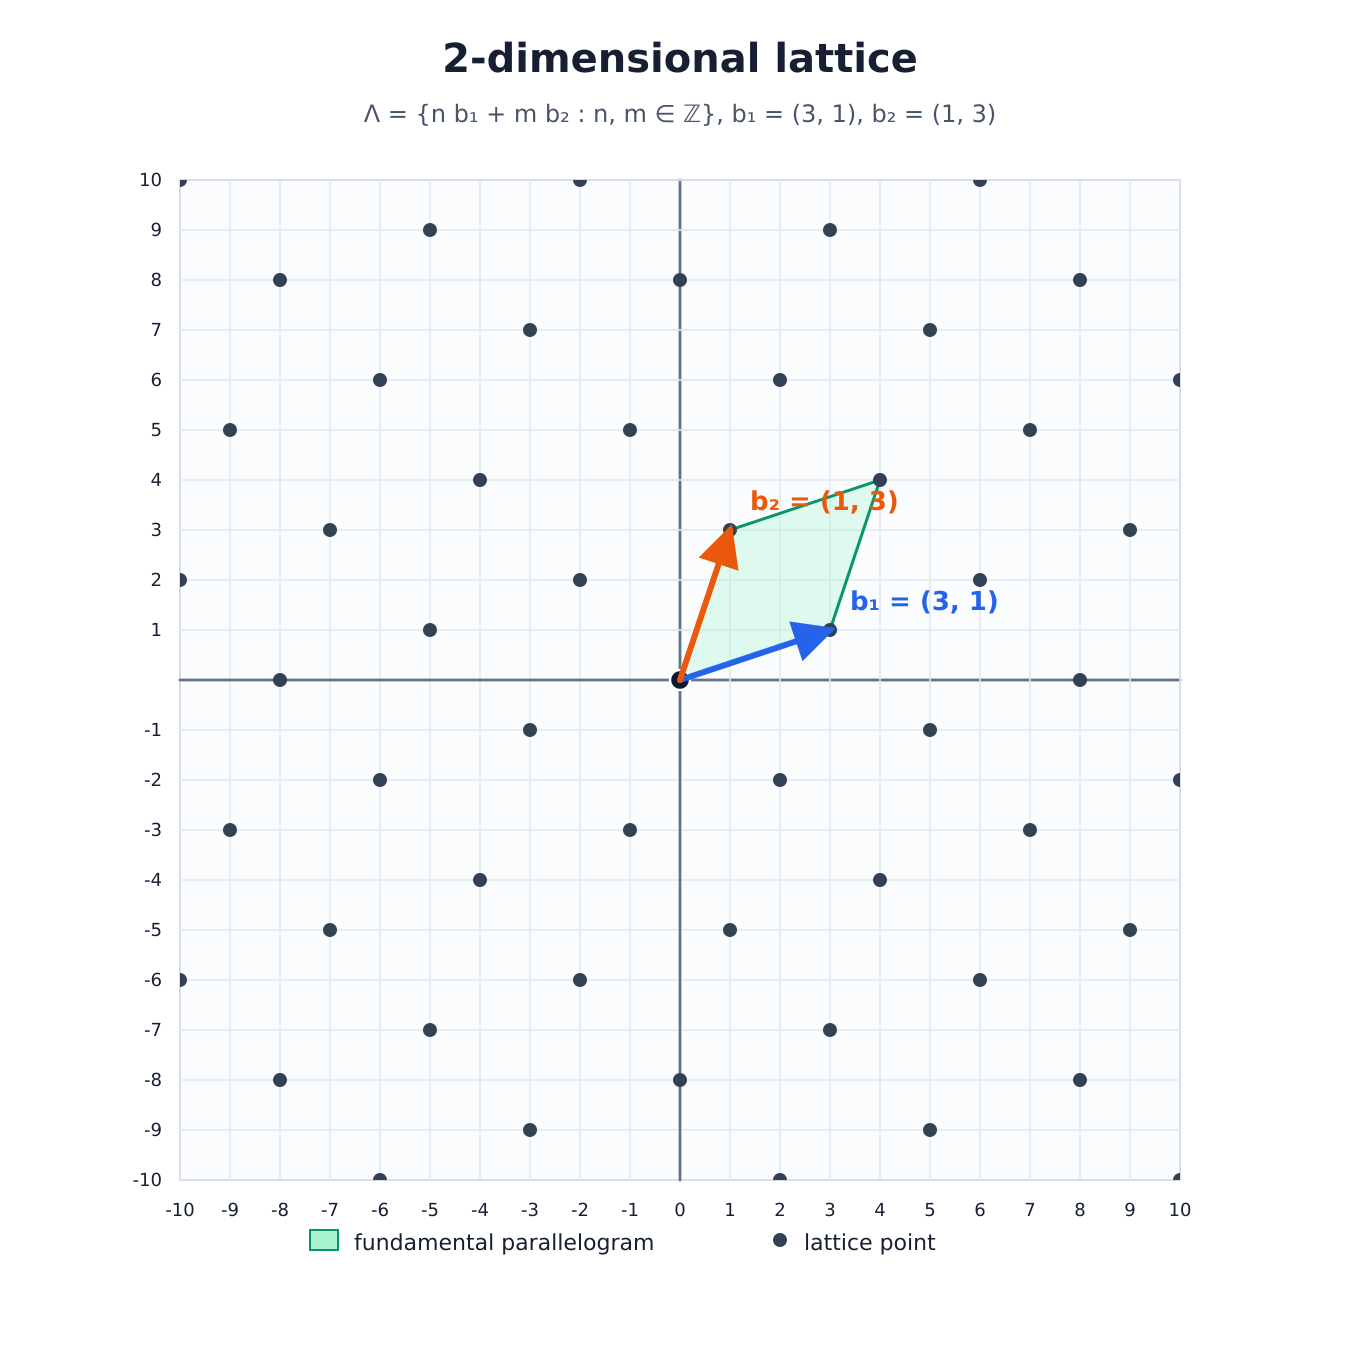
\includegraphics[width=9.5cm]{./2d-lattice}
\end{frame}

\begin{frame}{}
  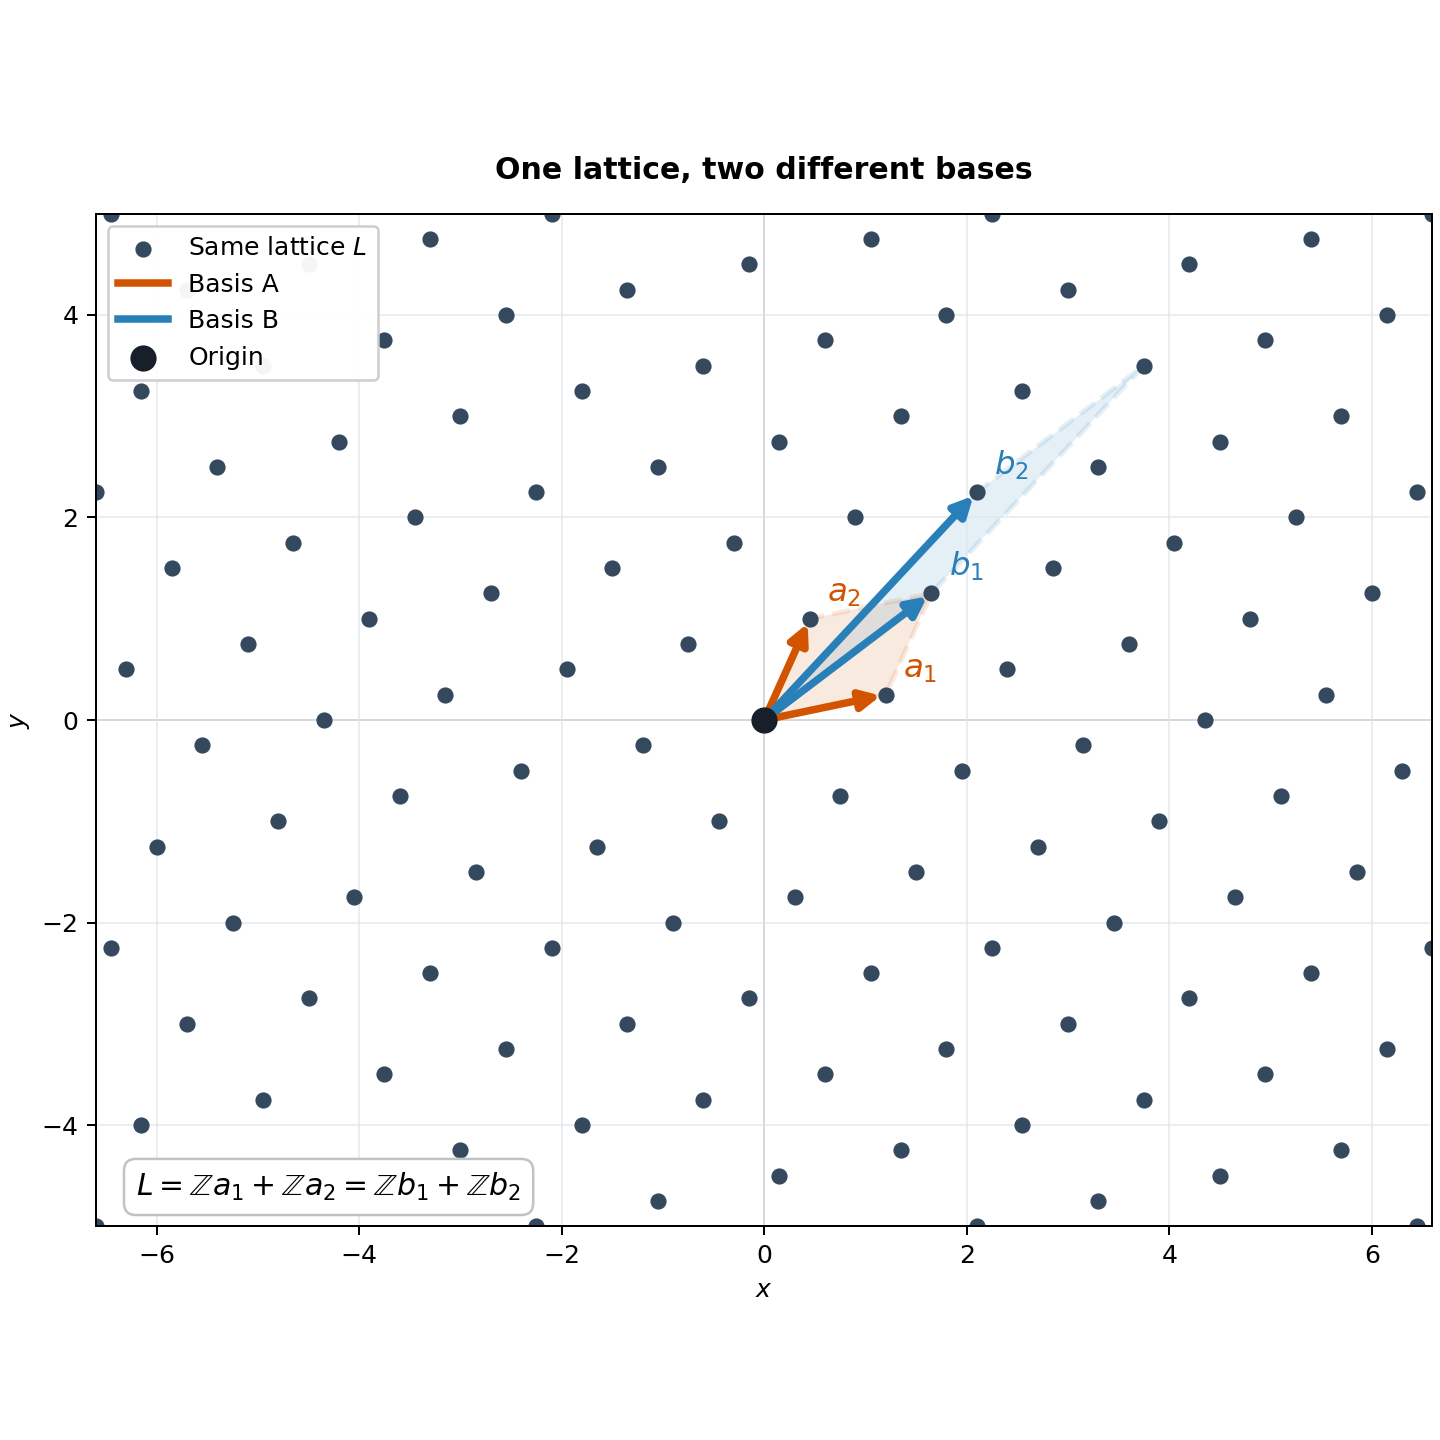
\includegraphics[width=9.5cm]{./two_bases_lattice}
\end{frame}

\begin{frame}{Lattice properties}
  a $n$-dimensional lattice $\Ll$ is
  \begin{enumerate}[i.]
    \item \emph{additive subgroup} of $\Rr^n$: $\Ll$ is the nonempty subset of $\Rr^n$ closed under vector addition (and substraction),\\
      $$\text{ie.}~ \forall x,y \in \Ll,~ -x, x+y \in \Ll$$
    \item \emph{discrete}: every $x \in \Ll$ has a neighborhood in $\Rr^n$ in which $x$ is the only lattice point.
  \end{enumerate}

  \pause

  \small{
  \begin{defn}[\emph{minimum} of a lattice $\Ll$]
    $$\lambda_1(\Ll) = min \{ ||x|| ~|~ x\in \Ll, x \neq 0 \}$$

    \pause

    \emph{Successive minima} $\lambda_i(\Ll)$: smallest radius $r$ s. th. $\Ll$ the $n$-dimensional ball of radius $r$ contains $i$ linearly independent lattice points.
    $$\lambda_1(\Ll) \leq \lambda_2(\Ll) \leq \cdots \leq \lambda_n(\Ll)$$
  \end{defn}
  }
\end{frame}

\begin{frame}{}
  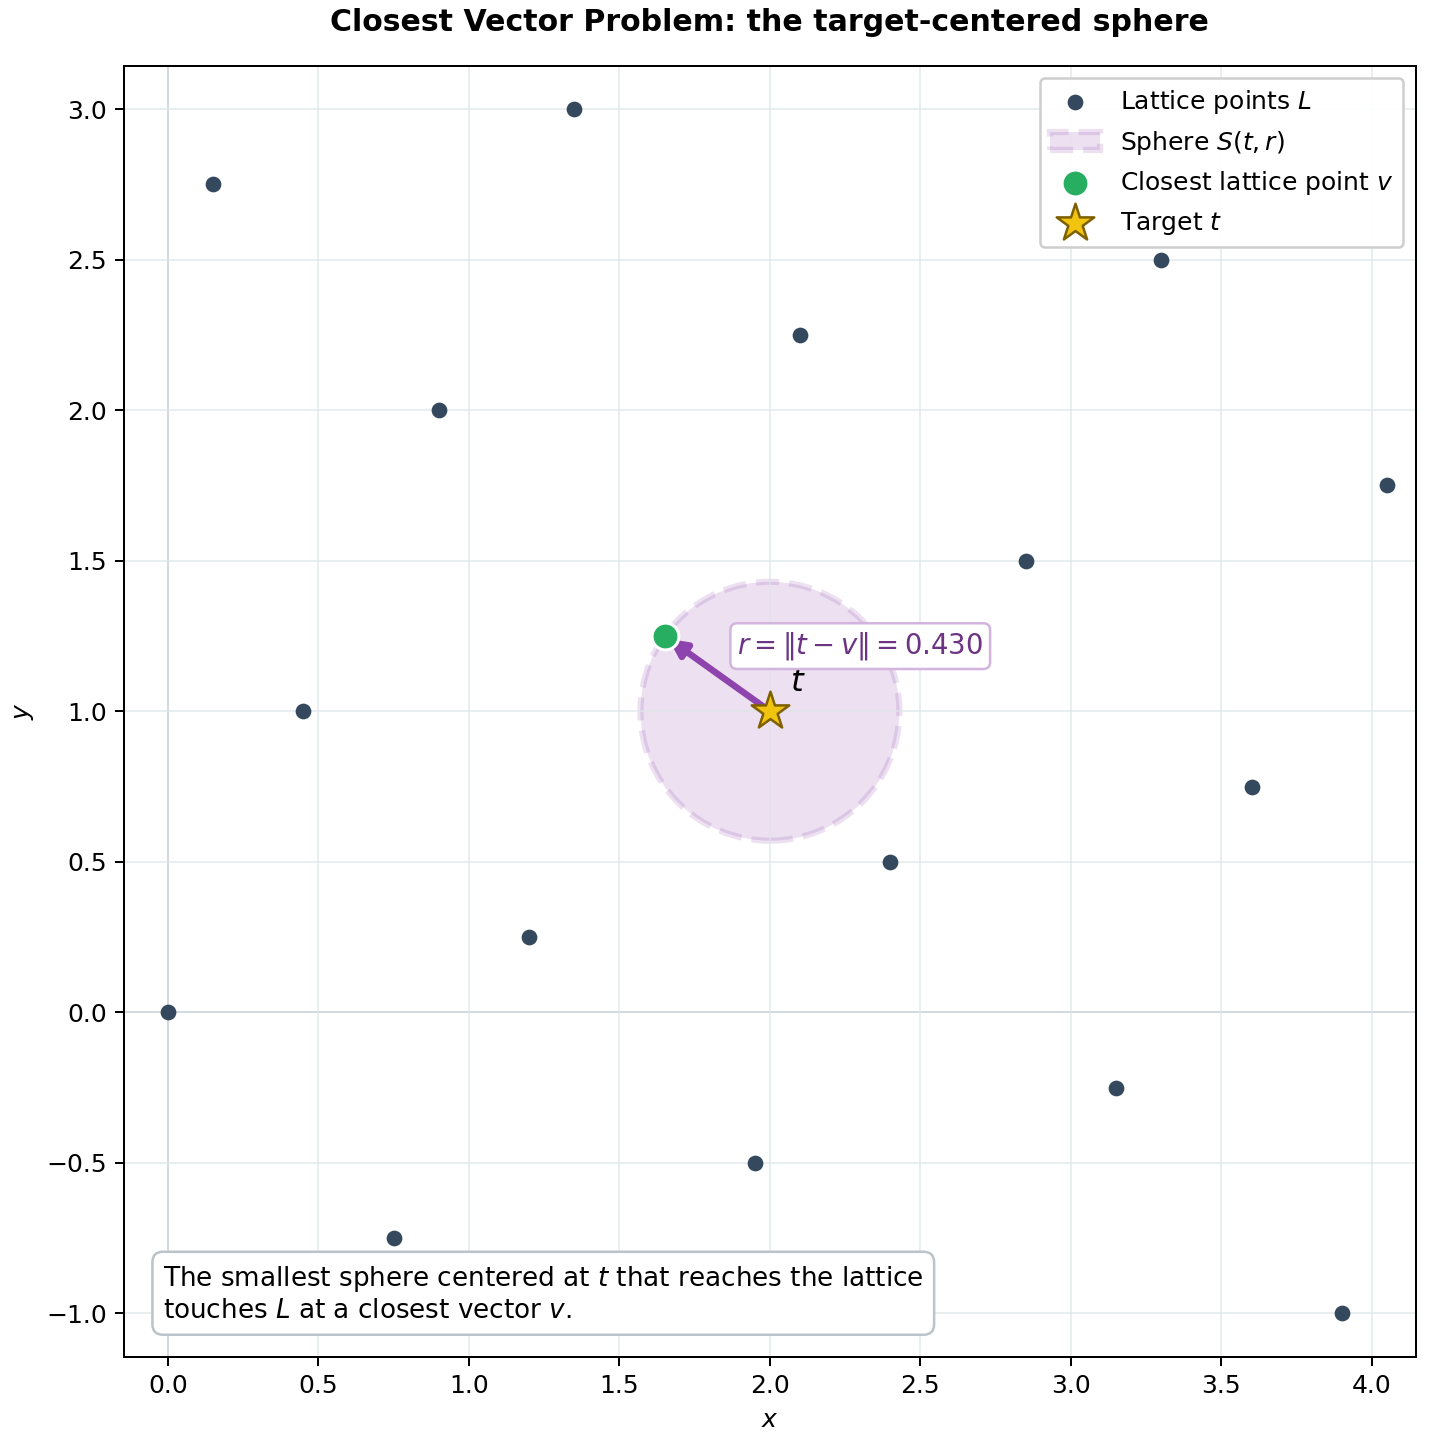
\includegraphics[width=9.5cm]{./cvp_sphere}
  % 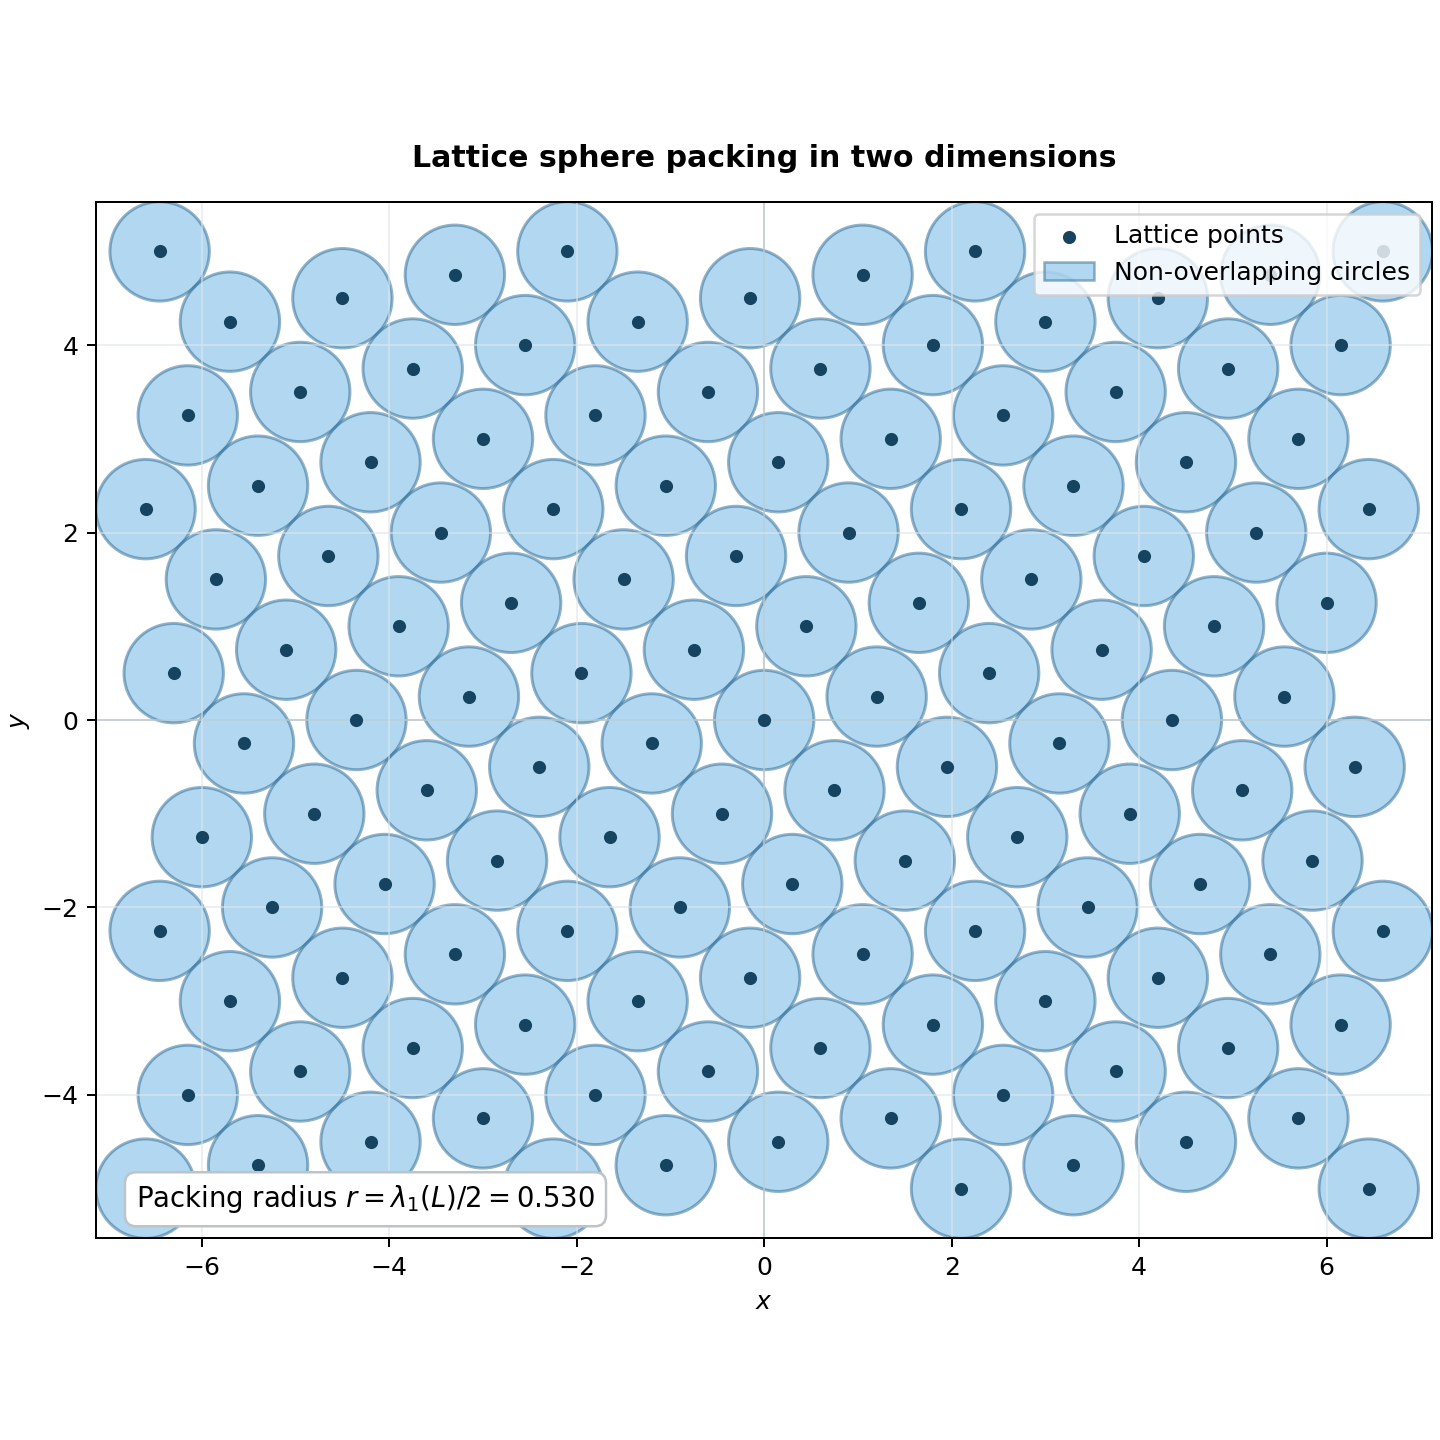
\includegraphics[width=9.5cm]{./sphere_packing} % TODO
\end{frame}

\begin{frame}{Lattice properties}
  \small{
  recall, a lattice:
  \vspace*{-0.7cm}
  $$\Ll(B) := B \cdot \Zz^n = \{ \sum_{i=1}^n z_i b_i ~|~ z_i \in \Zz^n \}$$

  \pause
  \vspace*{-0.4cm}
  \begin{itemize}
    \item $B = (b_1, \ldots, b_n) \in \Zz^{n \times n}$: basis matrix, finite description of the lattice (not the lattice itself)
    \item the matrix-vector product $Bz$ maps an integer coordinate vector $z \in \Zz^n$ into a lattice point in $\Zz^n$.
  \end{itemize}
  }

    \pause
  
  \vspace*{-0.4cm}
\begin{columns}[T]
  \begin{column}{0.65\textwidth}

  \small{
  \begin{itemize}
    \item since columns of $B$ are linearly independent (bcs they are a basis), every point of $\Ll(B)$ has a unique integer coordinate vector relative to the basis
    \begin{itemize}
      \item the lattice $\Ll(B)$ is the invariant set of points
      \item the basis $B$ is not unique
    \end{itemize}

  \vspace*{-0.3cm}
  \pause
  \item $B \in \Zz^{n \times n}$, $n$ vectors, each with $n$ coordinates $\Longrightarrow$ requires $\mathcal{O}(n^2)$ integers.
    \begin{itemize}
      \item only if we could have some better lattice structure to represent the lattice with fewer entries...
    \end{itemize}
  \end{itemize}
  }

  \end{column}

  \begin{column}{0.40\textwidth}
    \centering
    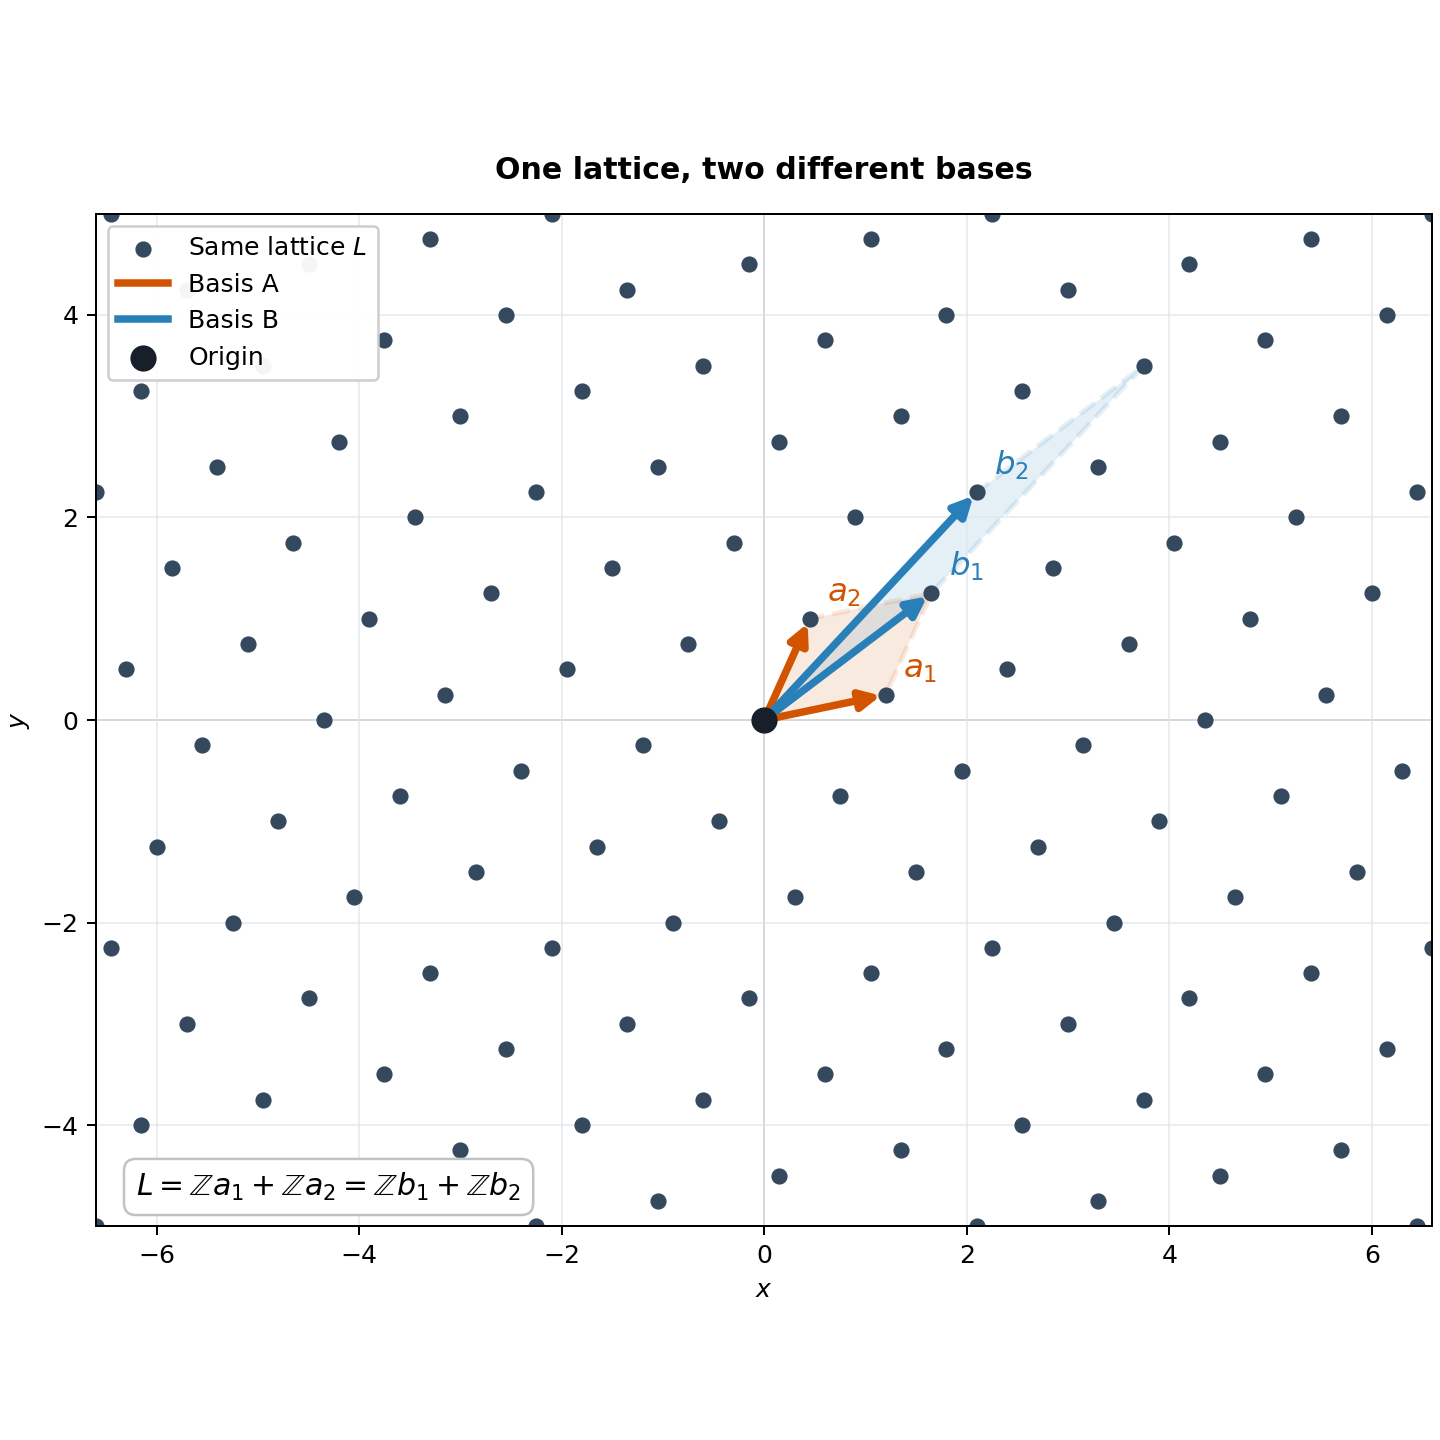
\includegraphics[width=\linewidth]{./two_bases_lattice}
  \end{column}
\end{columns}
\end{frame}


\begin{frame}{q-ary lattice}
  a full-rank lattice is q-ary if $q \Zz^d \subseteq \Ll \subseteq \Zz^d$

  $\Longrightarrow$ q-ary lattice is an infinite set of integer points, but membership depends only on the residue class modulo $q$
  $$\text{ie. if}~ x \in \Ll, ~\text{then}~ x + qz \in \Ll ~\forall z \in \Zz^d$$

  \pause

  Let $A \in \Zz^{n \times m}$ define the homomorphism
  \begin{align*}
    \psi_A: \Zz^m &\longrightarrow \Zz_q^n\\
    z &\longmapsto Az \pmod q
  \end{align*}

  \pause

  % image q-ary lattice:
  % $$\Ll_q(A) = \{ y \in \Zz^n ~|~ y=Az \mod q ~\text{for some}~ z \in \Zz_q^m \}$$
  % 
  % lattice generated by the rows of $A$.
  % \pause

  q-ary lattice:
  $$\Ll_q^{\perp}(A) = ker(\psi_A) = \{ z \in \Zz^m ~|~ Az = 0 \mod q \}$$
  contains all vectors that are orthogonal modulo $q$ to the rows of $A$.

  \scriptsize{
    The q-ary lattice generated by the rows of $A$:
    $$\Ll_q(A) = \{ y \in \Zz^m ~|~ y=A^Tz \mod q ~\text{for some}~ z \in \Zz_q^n \}$$
  }

  % TODO why q-ary is better? prev.slide says O(n^2) without q-ary, how with q-ary?
\end{frame}

\begin{frame}{Polynomial rings}
  \small{
    \begin{itemize}
      \item The NTRU paper (1996) introduced the usage of polynomial rings, which latter was ported over Ajtai work and other lattices, now is the general approach in Ring-SIS, Ring-LWE, Module-LWE, etc.

      \item Polynomial rings: represent an $n$-dimensional vector
      $(a_0,\ldots,a_{n-1}) \in \Zz_q^n$ as a single ring element (polynomial)
      $$a(X) = a_0 + a_1 X + \cdots + a_{n-1} X^{n-1} \in \Zz_q[X]/(X^n+1)$$
    \end{itemize}
  }

  \pause
  \small{
  \begin{itemize}
    \item[-] Addition:
      $a(x) + b(x) = \sum_{i=1}^d (a_i + b_i) X^i$
  \pause
    \item[-] Multiplication:
      $$a(X) \cdot b(X)
        = \left(
          \sum_{i=0}^{n-1}\sum_{j=0}^{n-1}
          a_i b_j X^{i+j}
        \right)
	\in \Zz_q[X]/(X^n+1)$$

	\hspace*{4em}Since $X^n=-1$ then $X^{n+k} = -X^k$\\
	  $\Longrightarrow~ \mathcal{O}(n^2)$ naively, $\mathcal{O}(n \log n)$ using NTT.
  \end{itemize}
  }
\end{frame}


\section[Hard problems]{Hard problems}

\begin{frame}{Incomplete Timeline}
  \begin{timeline}
    1978 \quad Knapsack cryptosystems attacked using lattice methods

    1996 \quad NTRU encryption

    2005 \quad Learning With Errors (LWE)

    2008 \quad Practical secure lattice-signature schemes

    2009 \quad Fully Homomorphic Encryption (FHE)

    2016 \quad NewHope (Ring-LWE KEM)

    2017 \quad Kyber (Module-LWE based) & Dilithium  (Module-LWE & Module-SIS based)

    2020s \quad standardiszation: ML-KEM (Kyber) and ML-DSA (Dilithium)
  \end{timeline}
\end{frame}


\begin{frame}{Hard problems in lattices - SVP and CVP}
  \small{
  \begin{itemize}
    \item In elliptic curve cryptography, we rely on the hardness of the Discrete Logarithm problem:\\
    \begin{adjustwidth}{2em}{0pt}
      given publicly known $g, p \in \mathbb{G}$, find privately known $x \in \Zz$ such that $p=g^x$.
    \end{adjustwidth}

    \item In lattice based cryptography, we rely on problems related to finding short vectors in the lattice.
  \end{itemize}
  }

  \pause
  \begin{defn}[SVP (Shortest Vector Problem)]
    find a shortest non-zero vector $x \in \Ll$, ie. that minimizes the Euclidean norm $||x||$, that is $\lambda_1(\Ll)=||x||$.
  \end{defn}

  \colorbox{gray!20}{Intuition:
    find the shortest possible jump from the origin to another dot
  }
  
  \pause
  \begin{defn}[CVP (Closest Vector Problem)]
    given a vector $y \in \Rr^n$ with $y \not\in \Ll$, find a nonzero vector $x \in \Ll$ that is closest to $y$, ie. that minimizes the Euclidean norm $||y-x||$.
  \end{defn}
  
  \colorbox{gray!20}{Intuition:
    find the grid dot that is closest to a given point (off the grid)
  }

\end{frame}

\begin{frame}
  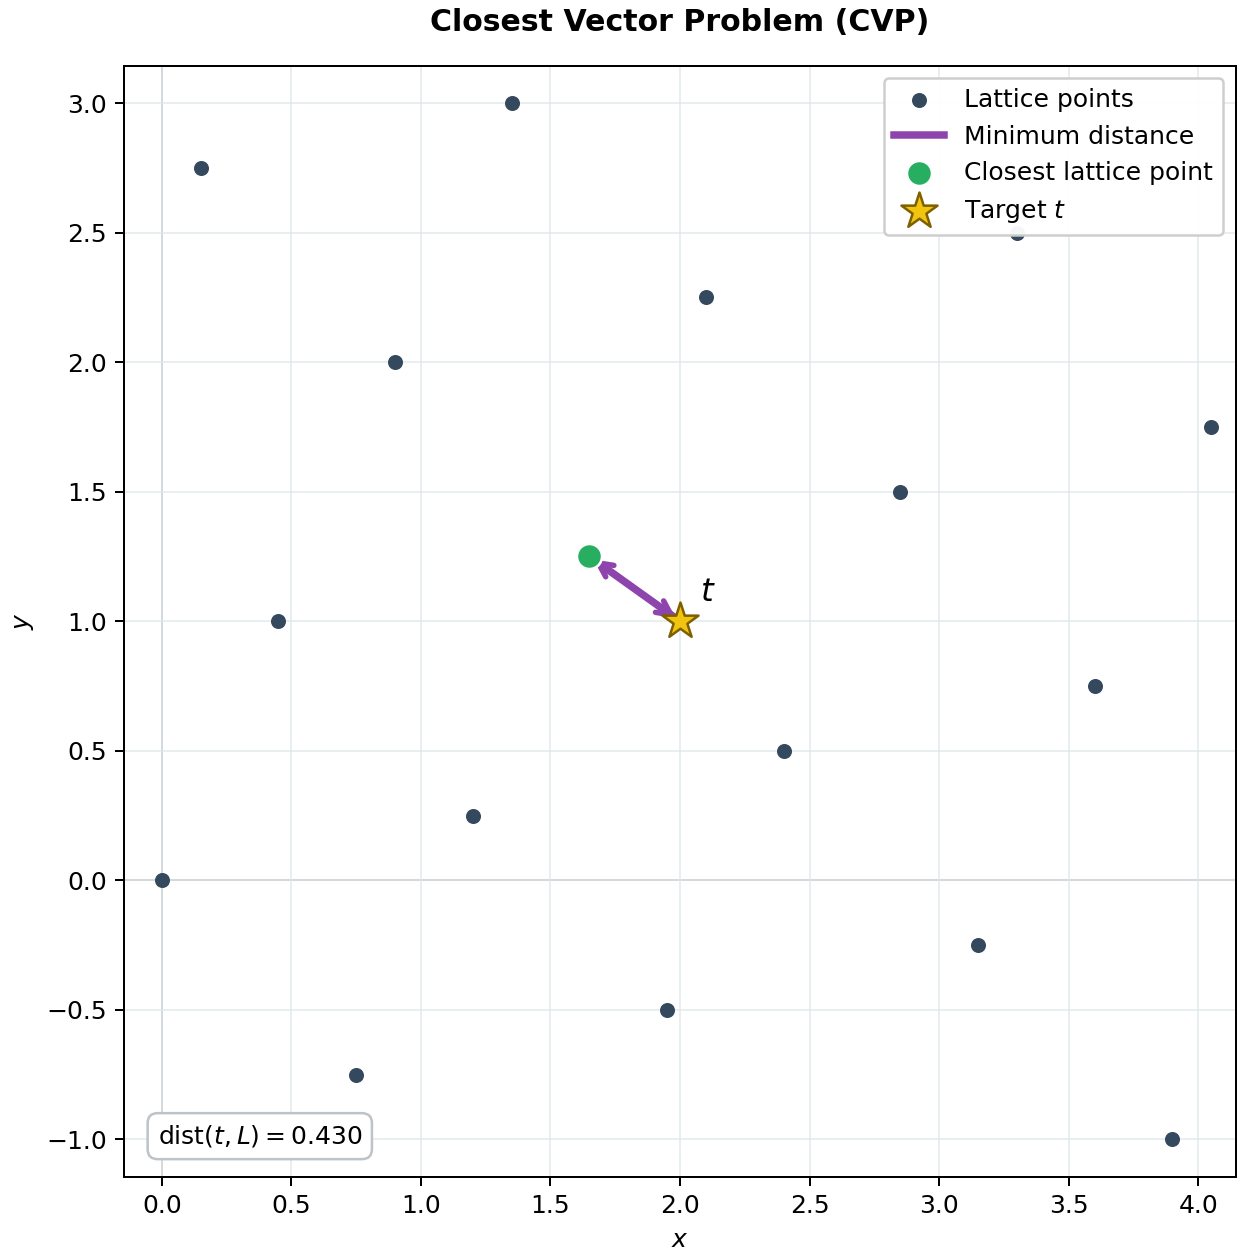
\includegraphics[height=\paperheight]{./cvp_2d}
\end{frame}

\begin{frame}{Why Lattices?}
  \begin{itemize}
    \item LLL algorithm is used to solve SVP and CVP.
    \begin{itemize}
      \item LLL (Lenstra–Lenstra–Lovász): polynomial time method used for lattice basis reduction, which transforms a given basis of a lattice into a new basis that is shorter and nearly orthogonal, which makes SVP and CVP easier to approximate or solve using subsequent algorithms.
      % \colorbox{gray!20}{Intuition:
      \begin{tcolorbox}[colback=gray!15, colframe=gray!15] Intuition:
	make the lattice basis less skewed. Same grid of points, just a simpler
	basis. We don't change the lattice, we change the coordinate system used to
	describe it. $\longrightarrow$ easier to solve SVP and CVP.
      % }
      \end{tcolorbox}
    \item improvement: BKZ reduction algorithm
    \end{itemize}

      \item Both SVP and CVP become computationally difficult (NP hard) as the
	lattice dimension $n$ grows (even on quantum computers)
  \end{itemize}
\end{frame}


\begin{frame}{NTRU}
  
  \begin{defn}[NTRU key recovery problem]
    Given $h(x)$, find ternary polynomials $f, g \in \mathcal{T}$ satisfying
    $$f(x) \cdot h(x) = g(x) \pmod q \in R_q$$
    Where $R_q = \Zz_q[X]/(X^n-1)$.
  \end{defn}
  
  \pause
  \begin{itemize}
    \item 1998, was first scheme using polynomial rings, which latter where approached as agebraically structured lattices
      \begin{itemize}
	\item "lattice-based" bcs recovering the small secret polynomials can be formulated and attacked as a lattice problem
	\item earlier lattice usage: in 1978, Knapsack cryptosystems targeted by lattice attacks
      \end{itemize}
    \item following the approach, in 2002, Micciano modified Ajtai's function to work over polynomial rings getting efficiency improvements
  \end{itemize}
\end{frame}

% TODO diagrams of SVP, CVP, SIS

\begin{frame}{Hard problems in lattices - SIS}
  \begin{defn}[SIS (Short Integer Solution)]
    given $q \in \Zz$ and matrix $A \in \Zz_q^{m \times n}$, find a non-zero short $z \in \Zz^n$ s.th.
    $$A \cdot z = 0 \pmod q$$

    \small{"short": $z \in \{B, B\}^n$ for some bound $B$, often $z \in \{-1, 0, 1 \}^n$.}
  \end{defn}

  \pause
  The set of all solutions to the SIS problem forms the (q-ary) lattice
  $$\Lambda^{\perp}_q(A) = \{ z \in \Zz^n ~|~ A \cdot z = 0 \pmod q \}$$
  where the SIS problem becomes the SVP for $\Lambda_q^{\perp}(A)$

  \small{
    \hspace*{2em}\colorbox{gray!20}{Intuition:
    find a short nonzero vector in the lattice $\Lambda^{\perp}_q(A)$
    }
  }

\end{frame}

\begin{frame}{}
  \begin{defn}[Ring SIS (Ring Short Integer Solution)]
    given a uniformly random matrix $A \in^R R_q^n$, with elements $a_i \in R_q$, find a non-zero integer vector $z \in R^n$ of norm $||z|| \leq \beta$ such that

    $$A z = \sum_i a_i \cdot z_i = 0 \in R_q$$
  \end{defn}

  \pause
  \begin{defn}[MSIS (Module Short Integer Solution)]
    given a uniformly random matrix $A \in^R R_q^{m \times n}$, with columns $a_i \in R_q^m$, find a non-zero integer vector $z \in R^n$ of norm $||z|| \leq \beta$ such that

    $$A z = 0 \in R_q^m$$
    $$ie.~ \sum_i a_{ij} \cdot z_j = 0 \in R_q, ~~for~ i=1, \ldots, m$$
  \end{defn}

  \pause
  Notice that Module-SIS is a Ring-SIS with $rank=1$ ($m=1$).
\end{frame}

\begin{frame}{}
  % TODO maybe rm these remarks
  \begin{itemize}
    \item without $||z|| \leq \beta$, it is easy to find a solution via \emph{Gaussian elimination}.
    \item $\beta < q$, because otherwise $z=(q, 0, \ldots, 0) \in R^m$ would always be a valid solution.
    \item $\beta$ and $m$ must be large enough so that a solution is guaranteed to exist, usually $\beta \geq \sqrt{\hat{m}}$ and $m \geq \hat{m}$ where $\hat{m}$ is the smallest integer greater than $n \log q$.
  \end{itemize}

  Again: overall when doing lattice-based cryptography, we will be interested into keeping the values \emph{short}, aka. of small norm.
  \pause
  (example of decomposing values to keep small norms when doing operations in
  cryptographic protocols (eg. in LaBRADOR))
\end{frame}

\begin{frame}{Hard problems in lattices}
  \begin{defn}[LWE (Learning With Errors)]
    choose a matrix $A \in^R \Zz_q^{m \times n}$, a secret vector $s \in^R \Zz_q^n$, and an error vector $e \in^R [-B, B]^m$. Let $b = As +e \pmod q \in \Zz_q^m$.

    Given the pair $(A, b)$, the goal is to recover $s$.
  \end{defn}
  Search-LWE \& Decisional-LWE problems.

  \pause
  For LWE samples, vector $b$ is relatively close to exactly one vector in the LWE lattice:
  \begin{align*}
  \Lambda_q(A) &= \{ A^T s ~|~ s \in \Zz_q^n \} + q \Zz^m\\
      &= \{ A^T s + qz ~|~ s \in \Zz_q^n, z \in \Zz^m \}
  \end{align*}

  \pause
  Observe: if $e=0$, is a system of linear equations, which can be efficiently determined using Gaussian elimination over $\Zz_q$. Hardness comes from the noise/error term $e \neq 0$ (and the norm bound).

  \pause
  Similarly as with SIS, we also have Ring-LWE and Module-LWE variants of LWE.
\end{frame}

\begin{frame}{Plain - Module - Ring}
  $$R_q = \mathbb{Z}_q[x]/(x^n+1)$$

  \small{
  $$
    \begin{array}{c|c|c}
      \text{Assumption} &
      \text{Public linear relation} &
      \text{Underlying algebra}
      \\ \hline
      \text{Plain LWE} &
      \mathbf{b} = A\mathbf{s} + \mathbf{e} \pmod q &
      A \in \mathbb{Z}_q^{m \times n}
      \\[0.5em]
      \text{Module-LWE} &
      \mathbf{b} = A\mathbf{s} + \mathbf{e} \pmod q &
      A \in R_q^{k \times k},
      \quad
      \mathbf{s},\mathbf{e},\mathbf{b} \in R_q^k
      \\[0.5em]
      \text{Ring-LWE} &
      b = as + e \pmod q &
      a,s,e,b \in R_q
    \end{array}
  $$
  $$
  \begin{array}{c|c|c}
    \text{Assumption} &
    \text{Public linear relation} &
    \text{Underlying algebra}
    \\ \hline
    \text{Plain SIS} &
    A\mathbf{z} = \mathbf{0} \pmod q,
    \quad
    \mathbf{z} \neq \mathbf{0},
    \quad
    \|\mathbf{z}\| \text{ small} &
    A \in \mathbb{Z}_q^{m \times n},
    \quad
    \mathbf{z} \in \mathbb{Z}^n
    \\[0.8em]
    \text{Module-SIS} &
    A\mathbf{z} = \mathbf{0} \pmod q,
    \quad
    \mathbf{z} \neq \mathbf{0},
    \quad
    \|\mathbf{z}\| \text{ small} &
    A \in R_q^{m \times n},
    \quad
    \mathbf{z} \in R^n
    \\[0.8em]
    \text{Ring-SIS} &
    a z = 0 \pmod q,
    \quad
    z \neq 0,
    \quad
    \|z\| \text{ small} &
    a \in R_q,
    \quad
    z \in R
  \end{array}
  $$
}


\end{frame}

\begin{frame}{Dual lattices}
  SIS lattice:
  $$\Ll^{\perp}(A) = \{ z \in \Zz^n ~|~ A \cdot z = 0 \pmod q \}$$

  LWE lattice:
  \begin{align*}
  \Ll(A) &= \{ A^T s ~|~ s \in \Zz_q^n \} + q \Zz^m\\
      &= \{ A^T s + qz ~|~ s \in \Zz_q^n, z \in \Zz^m \}
  \end{align*}


  \pause
  Dual of a lattice:
  $$\Ll^* = \{ y \in \Rr^m ~|~ \langle y, x \rangle \in \Zz ~\forall~ x \in \Ll \}$$

  ie. all vectors that measure lattice points with integers.

  \vspace{0.5cm}
  \pause
  SIS lattices and LWE lattices are dual to each other
  $$\Ll(A) = q \Ll^{\perp *}(A) ~~~\text{ie.}~~~ \frac{1}{q} \Ll(A) = \Ll^{\perp *}(A)$$

\end{frame}

\begin{frame}
  \hspace*{-0.8cm}
  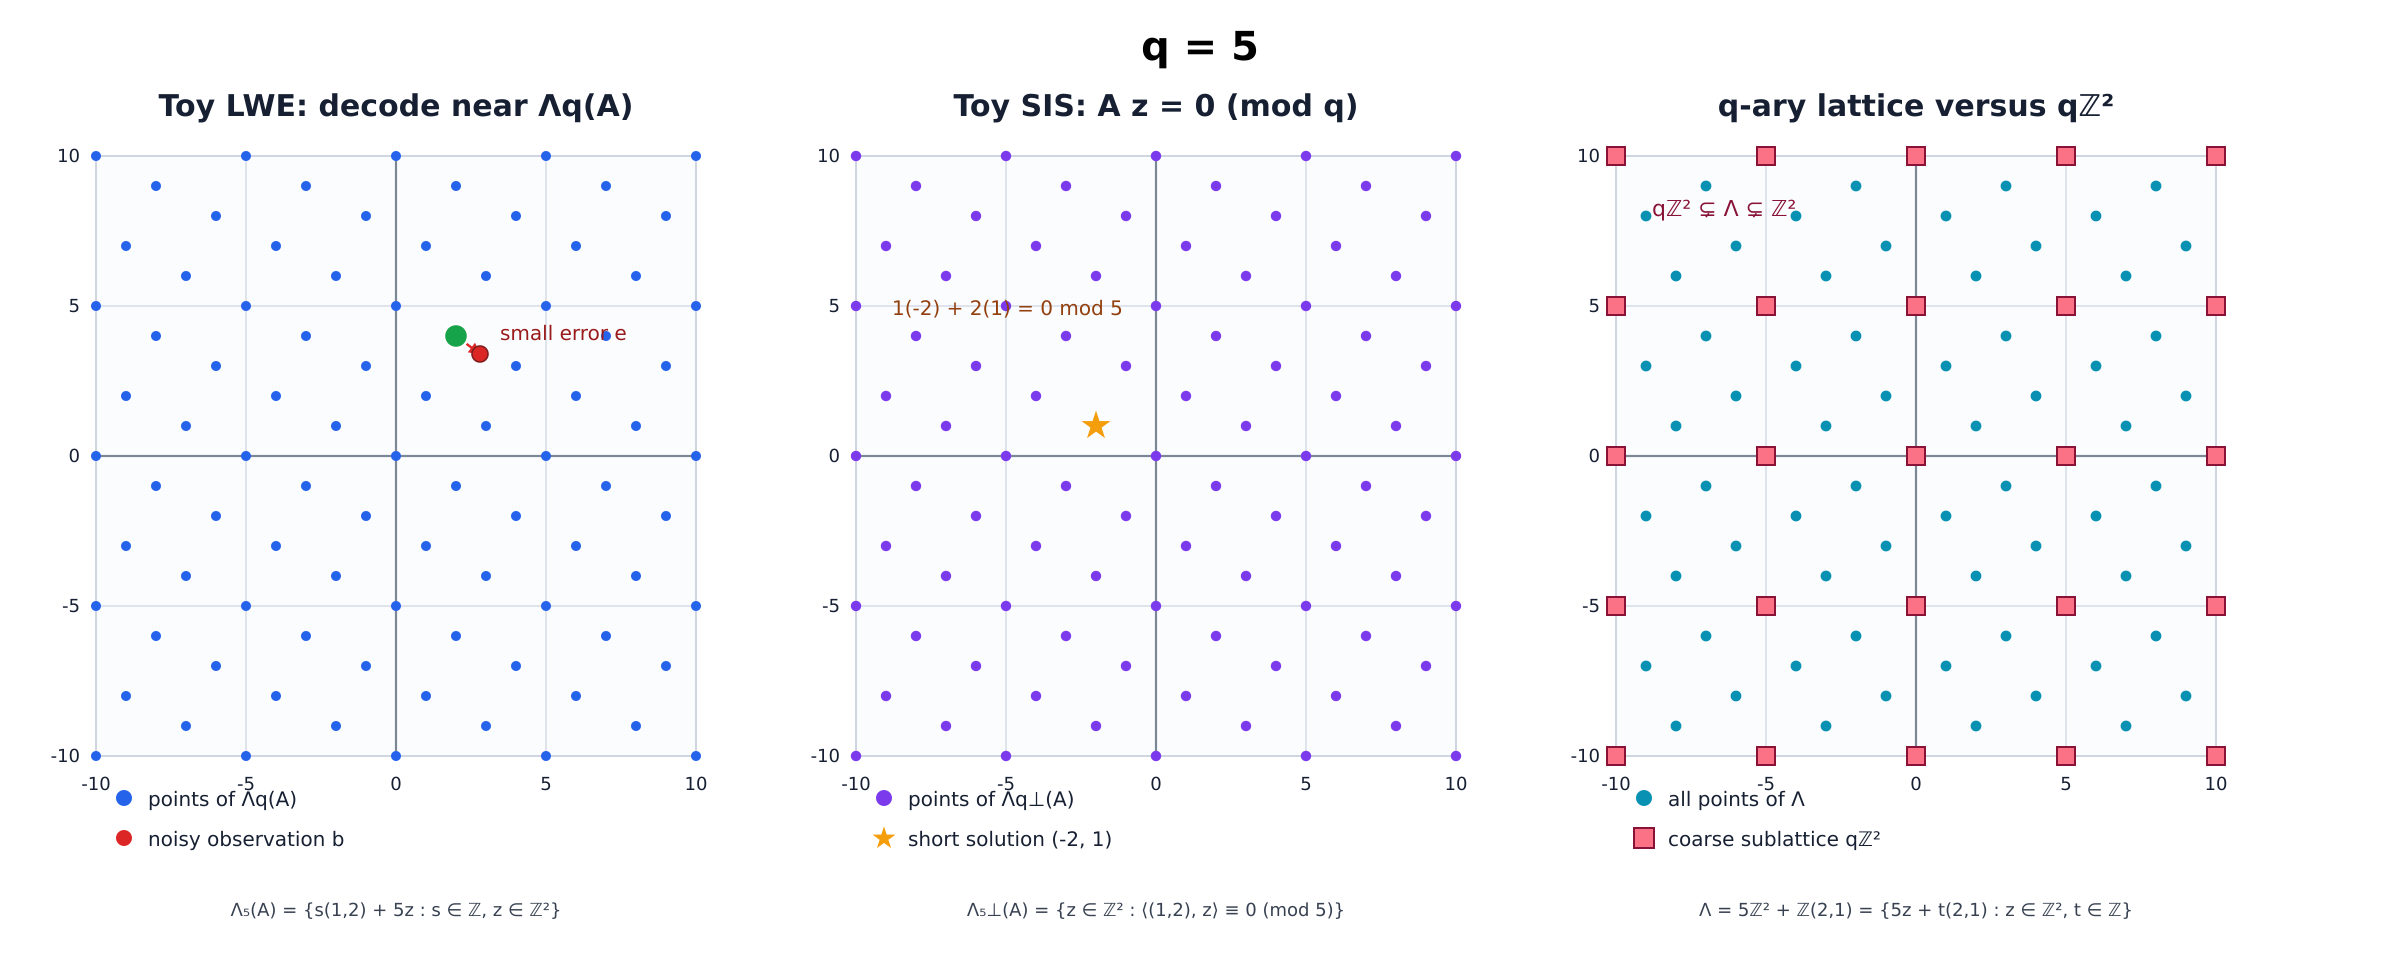
\includegraphics[width=\paperwidth]{./lattice_examples}
\end{frame}

\begin{frame}{Ajtai commitments}

  \begin{defn}[Ajtai commitemnt]
    For a public random matrix $A \in \Zz_q^{m \times n}$, embedding matrix $G \in \Zz_q^{m \times l}$ and a short random vector $r \in \{-B, B\}^n$ (for bound $B$), an Ajtai commitment to the message $x \in \Zz_q^l$ (bounded to $B$) is
    $$c = A r + G x \pmod q \in \Zz_q^n$$
  \end{defn}

  Observe that this is closely related to the SIS problem ($Az=0 \pmod q$), and it relies on its hardness.


\end{frame}

\section[Some cryptography]{Some cryptography}

\begin{frame}{Lattice-based cryptography}
  \begin{itemize}
    \item ML-KEM (Kyber): Key Encapulation Mechanism. ie. Alice encapsulates a (symmetric) key using Bob's public key
    \item ML-DSA (Dilithium): signature scheme
    \item FN-DSA (Falcon): signature scheme, based on NTRU
    \item LaBRADOR: SNARK scheme
    \item FHE (BFV, BGV, CKKS, TFHE)
  \end{itemize}
\end{frame}

\begin{mayberm}
\begin{frame}{ML-KEM (Kyber)}
  \scriptsize{
  \begin{itemize}
    \item KEM = Key Encapsulation Mechanism
    \begin{itemize}
      \item Alice encapsulates a (symmetric) key using Bob's public key
    \end{itemize}
  \item based on Module-LWE
  \end{itemize}
  }

$$R_q=\mathbb{Z}_q[X]/(X^{256}+1),  A\in R_q^{k\times k}$$

\textbf{Key generation:}
$$
\mathbf{s},\mathbf{e}\leftarrow\chi^k,
\qquad
\mathbf{t}=A\mathbf{s}+\mathbf{e}
$$

$$
pk=(A,\mathbf{t}),\qquad sk=\mathbf{s}
$$

\textbf{Encapsulation:}
$$
\mathbf{u}=A^T\mathbf{r}+\mathbf{e}_1,
\qquad
v=\mathbf{t}^T\mathbf{r}+e_2+\operatorname{Encode}(m)
$$

$$
c=(\mathbf{u},v),
\qquad
K=\operatorname{KDF}(m,c)
$$

\textbf{Decapsulation:}
$$
m'=\operatorname{Decode}\!\left(v-\mathbf{s}^T\mathbf{u}\right)
$$

Since
$$
v-\mathbf{s}^T\mathbf{u}
=
\operatorname{Encode}(m)
+\mathbf{e}^T\mathbf{r}
+e_2-\mathbf{s}^T\mathbf{e}_1,
$$
the message is recovered up to small noise.
\end{frame}
\end{mayberm}


\begin{frame}{ML-DSA signatures}
\end{frame}

\begin{mayberm}
\begin{frame}{Falcon signatures}
\end{frame}


\begin{frame}{LaBRADOR SNARK}
\end{frame}
\end{mayberm}

\section[Conclusions]{Conclusions}

\begin{frame}{Benchmarks}
  \centering
  % \small{
  \setlength{\tabcolsep}{4pt}
  \renewcommand{\arraystretch}{1.10}

  \textbf{Digital signatures}
  \vspace{0.05cm}

  \resizebox{0.88\textwidth}{!}{%
    \begin{tabular}{llll}
    \toprule
    \textbf{Scheme} &
    \textbf{Assumption} &
    \textbf{Public key size} &
    \textbf{Signature size} \\
    \midrule

    Falcon-512
      & NTRU lattice
      & $897$ B
      & $666$ B \\

    ML-DSA-44
      & Module-LWE / Module-SIS
      & $1.31$ KB
      & $2.42$ KB \\

    XMSS-SHA2-10-256
      & hash based, stateful
      & $64$ B
      & $2.50$ KB \\

    SLH-DSA-128s
      & hash based, stateless
      & $32$ B
      & $7.86$ KB \\

    ECDSA-secp256k1
      & elliptic curves
      & $33$ B
      & $64$ B \\

    \bottomrule
    \end{tabular}%
  }

  \vspace{0.20cm}

  \textbf{SNARKs / STARKs}
  \vspace{0.05cm}

  \resizebox{0.87\textwidth}{!}{%
    \begin{tabular}{lll}
    \toprule
    \textbf{Scheme} &
    \textbf{Assumption / technique} &
    \textbf{Proof size} \\
    \midrule

    Groth16
      & pairings / elliptic curves
      & $128$ B \\

    LaBRADOR
      & Module-SIS
      & $50$--$60$ KB \\

    Flock
      & binary fields + coding theory
      & $200$--$400$ KiB \\

    Binius64
      & binary fields + sumcheck
      & $200$--$500$ KiB \\

    Plonky2 & Plonk + FRI
      & $40$--$200$ KB \\

    Plonky3 / FRI-STARK
      & polynomial IOP + FRI
      & $1$--$3$ MiB \\

    \bottomrule
    \end{tabular}
  }
\end{frame}

\begin{frame}{Conclusions}
  \begin{itemize}
    \item not a single assumption: NTRU, SIS, R-SIS, M-SIS, LWE, R-LWE, M-LWE, $\ldots$
  \end{itemize}
\end{frame}


\end{document}
